\chapter{Grid-search results}

Although the minimal loss was achieved by the model with no L2-regularization, it is expected that training on more than 30 times the number of samples will require some regularization. In addition, the difference in performance between models with 88 and 64 is small and thus prefer a less complex model. The final model then has parameters 64 hidden units and L2-regularization parameter $1e-06$. 

\begin{figure}[h]
\centering
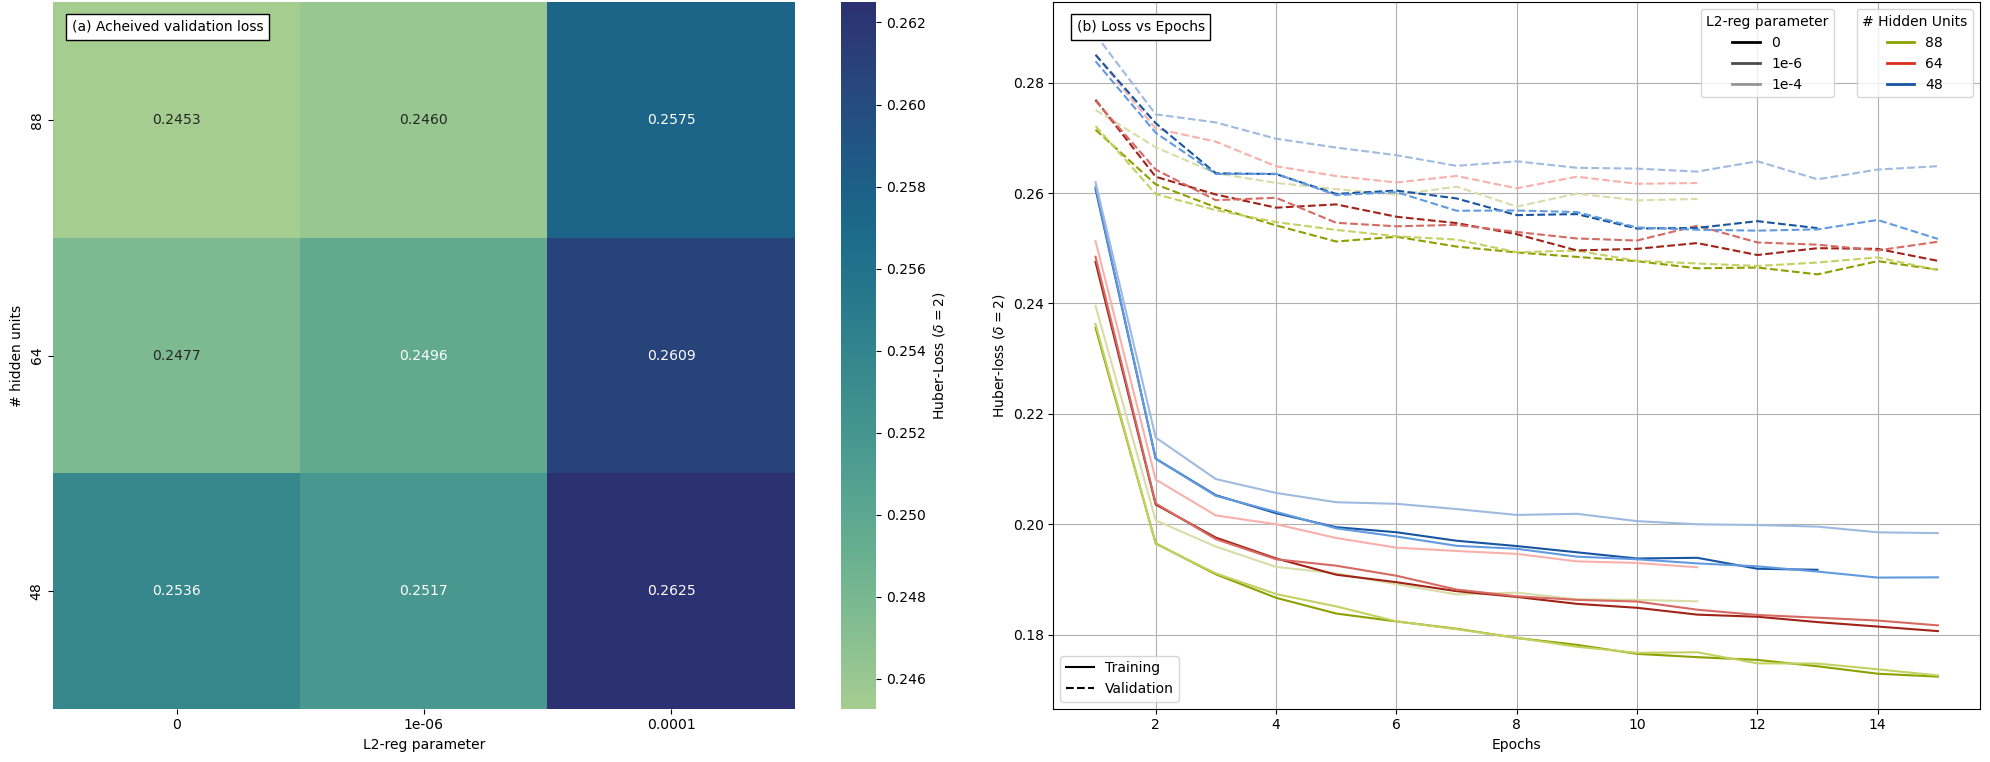
\includegraphics[width=\textwidth]{images/param_val.png}
\caption{Parameter validation results showing (a) the minimally achieved loss for each model instance and (b) the training and validation loss curves over epochs for each model instance.}
\end{figure}


%%% Local Variables: 
%%% mode: latex
%%% TeX-master: "MasterThesisSfS"
%%% End: 